%!TEX root = ../talk.tex

\section{Introduction}\label{sec:intro}

%%%

\frameinlbffalse

{
\usebackgroundtemplate{
\tikz[overlay,remember picture] \node[opacity=0.25, xshift=2.3cm, at=(current page.center)] {
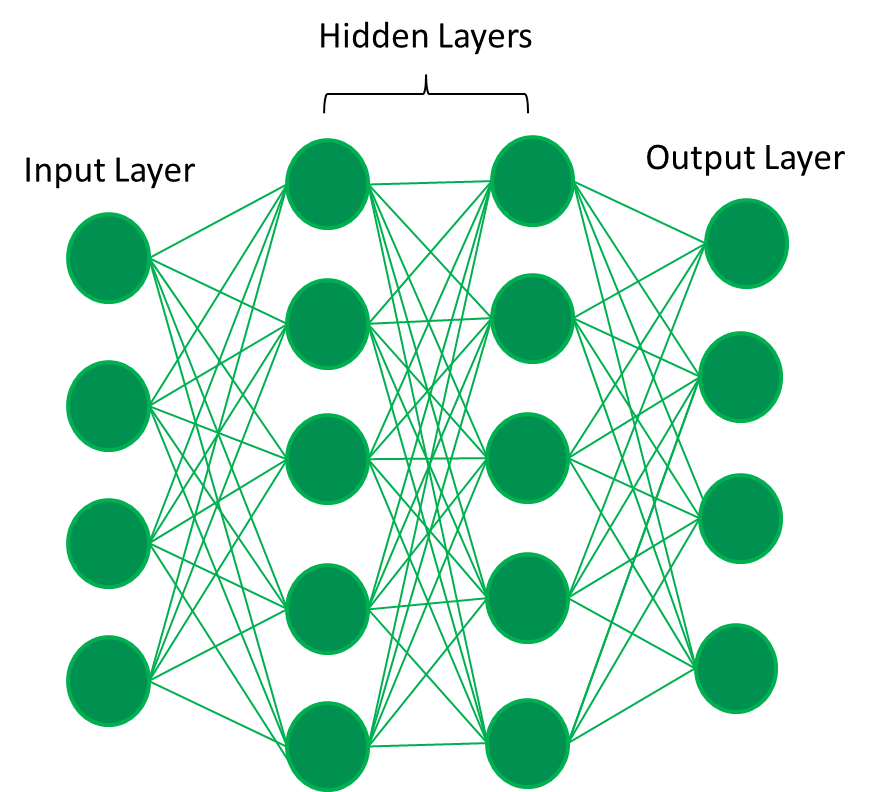
\includegraphics[width=0.65\paperwidth,height=0.5\paperwidth]{figures/genericDNN.png}
};}

\begin{frame}[plain]
\frametitle{\S\ref{sec:intro}. \insertsection}
\listofframes
\end{frame}
\addtocounter{framenumber}{-1} % this page does not count

}

\frameinlbftrue

%%%
\subsection{Background}
%%%

\begin{frame}
  \MyLogo
  \frametitle{Machine Learning}  
\small

\medskip

\structure{What is ML?}
\begin{itemize}

\item Unlike traditional numerical simulation, ``ML gives computers the ability to learn without being explicitly programmed'' {\footnotesize\color{DarkOrchid}[Samuel 1959]}

\item As a research field, ML explores the study and construction of algorithms that can {learn} from and {make predictions} on \alert{data}

\item Fourth paradigm, big data, Internet of things, artificial intelligence, ...

\end{itemize}

\structure{General Tasks of ML:}

\begin{itemize}

\item Classification: Inputs are divided into two or more classes, and the learner must produce a model that assigns unseen inputs to one or more of these classes

\item Clustering: Inputs are divided into several groups. Unlike in classification, the groups are not known beforehand, making this an unsupervised task

\item Regression: Similar to classification, but the outputs are continuous

\item Density estimation, dimensionality reduction, ...

\end{itemize}

\vfill
\begin{center}
{\color{red} \scriptsize
Deep Learning, by I. Goodfellow, Y. Bengio, and A. Courville, Chinese version available online

https://github.com/exacity/deeplearningbook-chinese
}
\end{center}
\end{frame}

%%%

\begin{frame}
  \MyLogo
  \frametitle{ML Software Packages}  

\begin{figure}[htbp] %  figure placement: here, top, bottom, or page
   \centering
   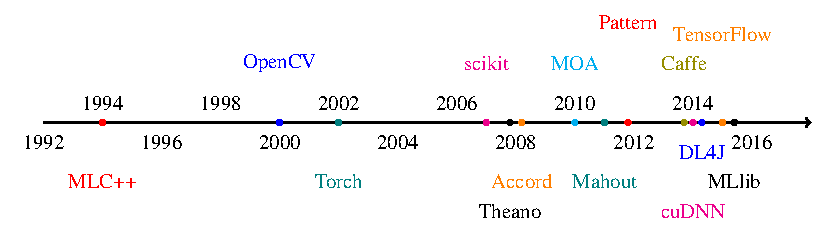
\includegraphics[width=1.0\linewidth]{figures/ML.pdf} 
\end{figure}

\begin{itemize}
\item[\raisebox{-0.4ex}{\alert{\HandRight}}] Other worth-noting packages: 
	\begin{itemize}
	\item CNTK/DMTK (Microsoft): 
		\begin{itemize}
		\item[-] Support Windows/Linux, no official OS X support
		\item[-] Provide C++/Python frontend
		\end{itemize}
	\item Neon (Nervana \& Intel)
	\item Caffe2 (Facebook)
	\item PyTorch (\alert{beta})
	\end{itemize}
\end{itemize}

\vfill
\begin{center}
{\color{red} \scriptsize
Tour of TensorFlow, by Peter Goldsborough, arXiv, 2016}
\end{center}

\end{frame}

%%%
\subsection{DL engines}
%%%

\begin{frame}
  \MyLogo
  \frametitle{Deep Learning}  

\small

\begin{mdframed}[style=mystyle2]
Deep Learning has been introduced with the objective of moving ML closer to one of its original goals---AI. The main motivations includes:
%
\begin{itemize}\scriptsize\setlength\itemsep{0.2em}
\item Insufficient depth can hurt
\item The brain has a deep architecture
\item Cognitive processes seem deep
\end{itemize}
\end{mdframed}

\medskip

\begin{columns}

\column{.49\textwidth}
{\color{blue}Pros:}
\begin{itemize}\setlength\itemsep{0.2em}
\item conceptually simple
\item nonlinear 
\item highly flexible and configurable
\item learned features can be extracted
\item can be fine-tuned with more data
\item efficient for multi-class problems
\item world-class at pattern recognition
\end{itemize}

\column{.51\textwidth}
{\color{red}Cons:}
\begin{itemize}\setlength\itemsep{0.2em}
\item hard to interpret 
\item theory not well understood
\item slow to train and score
\item overfits, needs regularization
\item more parameters
\item inefficient for categorical variables
\item data hungry, learns slowly 
\end{itemize}
\end{columns}

\begin{center}
{\color{red} \scriptsize
https://www.slideshare.net/0xdata/transform-your-business-with-ai-deep-learning-and-machine-learning}
\end{center}

\end{frame}

%%%
\subsection{General comparison}
%%%

%%%

\begin{frame}
  \MyLogo
  \frametitle{Goal of This Study}  
\small

\medskip
\structure{What is our purpose?}
\begin{itemize}
\item Solving practical problems from various applications (user interface)
\item Developing algorithms and optimizing implementation (development)
\item Theoretical analysis for machine learning, ...
\end{itemize}

\structure{How to use a ML package?}
\begin{itemize}
\item Train models on large data set on high-performance computing platforms
\item Deploy applications on various computing platforms
\end{itemize}

\structure{What we want for a ML package?}
\begin{itemize}
\item Easy to build new tasks and new network structures (less steep learning curve)
\item Easy for debugging (with good documentation, support, and large community)
\item Good performance and scalability
	\begin{itemize}
	\item[-] Multicore CPU
	\item[-] Single or multiple GPU(s)
	\item[-] Cluster
	\end{itemize}
\end{itemize}

\end{frame}

%%%

\begin{frame}
  \MyLogo
  \frametitle{DL Engines: Basic Information}  
\small

\renewcommand{\multirowsetup}{\centering} 
\begin{table}[htdp]
\begin{center}
\begin{tabular}{|c|c|c|c|c|c|} \hline
\rowcolor{GreenYellow}
Viewpoint &Torch       &Caffe   & TensorFlow  & MXNet \\ \hline
Released      & 2002      &2013               &2015                & 2015                    \\ \hline
 \multirow{3}{4em}{Main \\ Developers}
 & Facebook,        &\multirow{3}{5em}{BAIR \\ BVLC}  &\multirow{3}{3em}{Google} &\multirow{3}{*}{DMLC}   \\ 
 &Twitter,            & & &    \\
 &Google, ...       & & &  \\ \hline 
\multirow{2}{4em}{ Core \\ Languages}     
& \multirow{2}{3em}{ C/Lua }      
&\multirow{2}{4em}{ C++}
&\multirow{2}{4em}{ C++\\Python}
&\multirow{2}{6em}{ C++}  \\ 
&   &    & &      \\ \hline
\multirow{2}{4em} {Supported \\Interface }    
& \multirow{2}{3em}{ Lua }      
&\multirow{2}{5.5em}{ C++/Python \\ Matlab}
&\multirow{2}{6.2em}{ \alert{Python}/C++/\alert{R} \\ Java/Go/...}  
&\multirow{2}{6.2em}{ C++/\alert{Python}/\alert{R} \\ Matlab/Julia/...}\\  
&   &    & &      \\ \hline           
 \multirow{2}{4em}{ License }     
& \multirow{2}{3em}{BSD}      
&\multirow{2}{4em}{BSD}
&\multirow{2}{4em}{Apache}
&\multirow{2}{6em}{Apache}  \\ 
&   &    & &      \\ \hline
\end{tabular}
\end{center}
\label{default}
\end{table}%

\vskip -10pt
{\scriptsize
\begin{itemize}\setlength\itemsep{0.5em}
\item BAIR, Berkeley Artificial Intelligence Research Lab 
\item BVLC, Berkeley Vision and Learning Center
\item DMLC, Distributed (Deep) Machine Learning Community, supported by Amazon, Intel, Microsoft, nVidia, Baidu, ...
\end{itemize}
}

\vfill
\begin{center}
{\color{red}\scriptsize
http://blog.revolutionanalytics.com/2016/08/deep-learning-part-1.html
}
\end{center}

\end{frame}

%%%

\begin{frame}
  \MyLogo
  \frametitle{DL Engines: Performance}  
\small

\renewcommand{\multirowsetup}{\centering} 
\begin{table}[htdp]
\begin{center}
\begin{tabular}{|c|c|c|c|c|c|} \hline
\rowcolor{GreenYellow}
Viewpoint &Torch7       &Caffe  & TensorFlow & MXNet  \\ \hline
  \multirow{2}{4em}{Pretrained \\ Models}      
  &  \multirow{2}{4em} {Yes}      
  &  \multirow{2}{4em}{Yes}                             
  &  \multirow{2}{4em}{No}                   
  &  \multirow{2}{4em}{Yes}\\ 
  &  &   &   & \\ \hline
\multirow{2}{4.5em}{High-level \\ Support}     
& \multirow{2}{*}{Good}      
&\multirow{2}{*}{ Good}
&\multirow{2}{*}{ Good}
&\multirow{2}{*}{ Good}  \\ 
&   &    & &      \\ \hline
 \multirow{2}{4em}{Low-level \\ Operators}
 &\multirow{2}{4em}{Good}
 &\multirow{2}{*}{Good }     
 &\multirow{2}{*}{Fairly good}
 &\multirow{2}{*}{Increasing fast}\\ 
 &       &    &  &  \\ \hline 
\multirow{2}{4em} {Speed \\ One-GPU }    
& \multirow{2}{*}{ Great }      
&\multirow{2}{*}{Great} 
&\multirow{2}{*}{Good}
&\multirow{2}{*}{Good} \\  
&   &    & &      \\ \hline          
\multirow{2}{5em} {Memory \\ Management}    
& \multirow{2}{*}{ Great }      
&\multirow{2}{*}{Great}
&\multirow{2}{*}{\alert{Not so good}}
&\multirow{2}{*}{ Excellent}  \\  
&   &    & &      \\ \hline            
\multirow{2}{3.5em} {Parallel \\ Support}    
& \multirow{2}{5.em}{Multi-GPU}      
&\multirow{2}{5.em}{Multi-GPU}
&\multirow{2}{5.em}{Multi-GPU} 
&\multirow{2}{5em}{Distributed} \\  
&   &    & &      \\ \hline            
\multirow{2}{3.5em} {Coding \\ Style}    
& \multirow{2}{5.em}{Imperative}      
&\multirow{2}{5.em}{Declarative}
&\multirow{2}{5.em}{Declarative} 
&\multirow{2}{5em}{Mixed} \\  
&   &    & &      \\ \hline
\multirow{2}{3.5em} {GitHub \\ Watching}    
& \multirow{2}{5.em}{649/268}      
&\multirow{2}{5.em}{1856}
&\multirow{2}{5.em}{4939} 
&\multirow{2}{5em}{887} \\  
&   &    & &      \\ \hline
\end{tabular}
\end{center}
\label{default}
\end{table}%

\end{frame}

%%%
\subsection{Test setting}
%%%

\begin{frame}
	\MyLogo
	\frametitle{Hardware Platforms}  

\smallskip 

\begin{itemize}

\item CPU: one quad-core desktop CPU (Intel i7-3820 CPU
		@3.60GHz) and two 8-core server-grade CPUs (Intel
		Xeon CPU E5-2630 v3 @2.40GHz)
		
\item GPU: GTX 1080 @1607MHz with
		Pascal architecture, and Telsa K80 @562MHz with Kepler
		architecture 
	\end{itemize}
	
\begin{figure}[htbp] 
	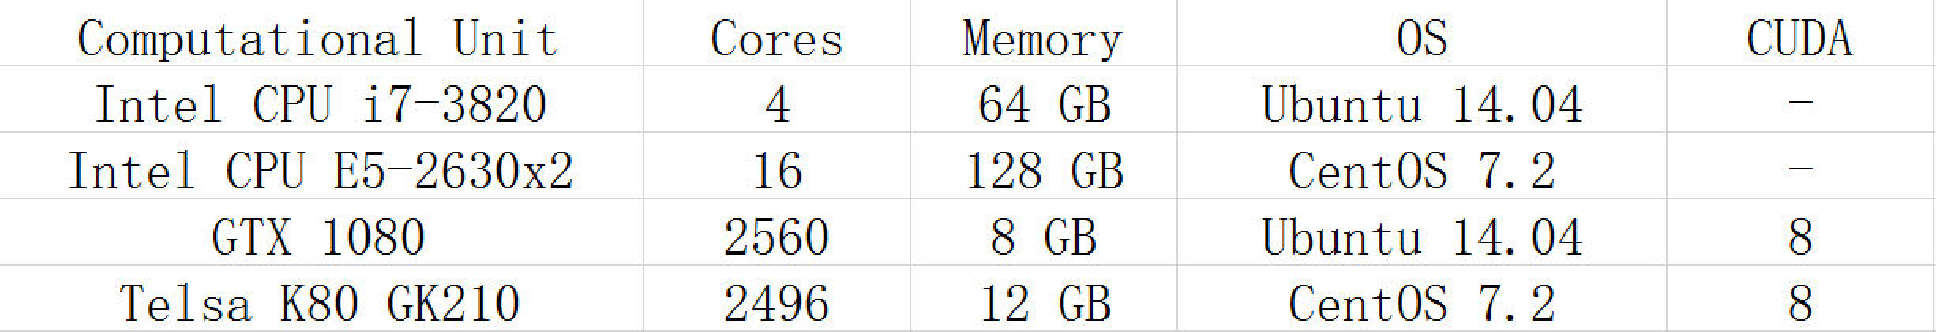
\includegraphics[height=1.3in]{figures/platforms.pdf} 
	\caption{The experimental hardware settings for numerical tests}
\end{figure}
	
\begin{center}
{\color{red} \scriptsize
Benchmarking State-of-the-Art Deep Learning Software Tools, by S.-H. Shi, et al., arXiv, 2017}
\end{center}

\end{frame}

%%%

\begin{frame}
  \MyLogo
  \frametitle{Neural Networks and Test Data Sets}  

\medskip

\begin{itemize}

\item A large fully-connected neural network (\alert{FCN-S}) with around 55 million parameters is used to evaluate the performance of FCN

\item The classical AlexNet (\alert{AlexNet-S}) is used as an representative of CNN

\item A smaller FCN (\alert{FCN-R}) is constructed for MNIST data set

\item An AlexNet (\alert{AlexNet-R}) architecture is used for Cifar10 data set

\item For RNNs, considering that the main computation complexity is related to the length of input sequence, 2 LSTM layers with input length of 32.

\end{itemize}

\begin{figure}[htbp] 
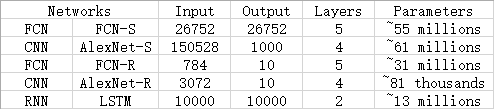
\includegraphics[height=1in]{figures/models.png} 
\caption{The experimental setup of neural networks for synthetic and real data}
\end{figure}
	
\end{frame}

